\chapter{Especies químicas naturales y sintéticas}\label{ch:g10:chemical-species}

Una cucharada de helado de vainilla. Su aroma puede venir de las vainas
negras de una orquídea tropical, recolectadas, curadas y maceradas en
alcohol durante meses; o puede venir de una fábrica que obtiene el aroma
a partir de pasta de madera o de petróleo. Si se prueban uno al lado del
otro, el aroma principal es el mismo, y con razón: la \omterm{def:g7:atoms-and-molecules:molecule}{molécula} que sabe a
vainilla, la vainillina, es exactamente la misma \omterm{def:g7:atoms-and-molecules:molecule}{molécula}, se haya
obtenido de una forma o de la otra. Este capítulo muestra cómo los
químicos extraen una especie de una planta, cómo la fabrican y cómo
comprueban que lo que tienen es lo que creen tener.

\begin{recall}
Una \omterm{def:g6:pure-substances-and-mixtures:species}{especie química} es una clase concreta de sustancia; una \omterm{def:g6:pure-substances-and-mixtures:pure-substance}{sustancia
pura} contiene una sola especie y tiene constantes fijas, como sus
temperaturas de fusión y de ebullición (\cref{ch:g6:pure-substances-and-mixtures}).
Los líquidos son \omterm{def:g6:solutions-and-solubility:miscible}{miscibles} o \omterm{def:g6:solutions-and-solubility:miscible}{inmiscibles}, y cada \omterm{def:g6:solutions-and-solubility:solute}{soluto} tiene su propia
\omterm{def:g6:solutions-and-solubility:solubility}{solubilidad} en cada \omterm{def:g6:solutions-and-solubility:solute}{disolvente} (\cref{ch:g6:solutions-and-solubility}).
La \omterm{def:g7:identifying-substances:chromatography}{cromatografía en papel} separa los colorantes de una \omterm{def:g6:pure-substances-and-mixtures:mixture}{mezcla}
(\cref{ch:g7:identifying-substances}).
\end{recall}

\begin{omfigure}
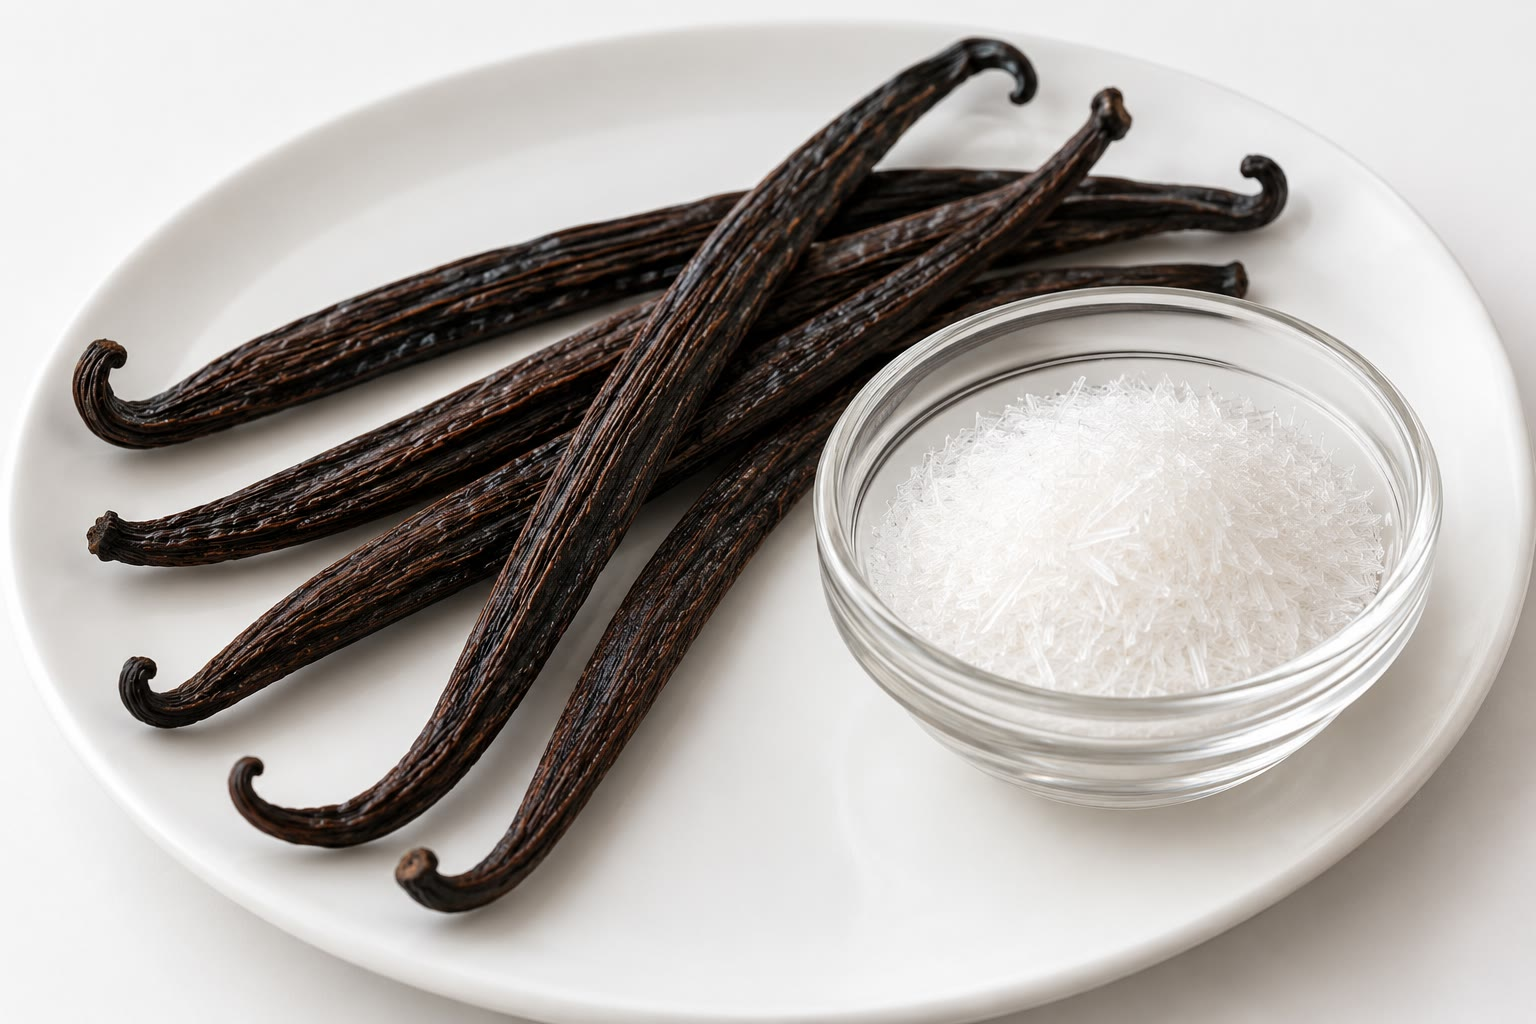
\includegraphics[width=0.55\linewidth]{images/book1/ai/g10-vanilla.jpg}

{\small Vainas de vainilla y cristales blancos de vainillina: la misma
\omterm{def:g7:atoms-and-molecules:molecule}{molécula}, de una planta o de una fábrica.}
\end{omfigure}

\section{Especies naturales y sintéticas}

\begin{definition}[Especies naturales y sintéticas]\label{def:g10:chemical-species:natural}
Una \emph{especie natural}\index{especie natural} es una \omterm{def:g6:pure-substances-and-mixtures:species}{especie química}
fabricada por un ser vivo o que se encuentra tal cual en la naturaleza.
Una \emph{especie
sintética}\index{especie sintetica@especie sintética} la fabrican los químicos a partir de
otras especies mediante \omterm{def:g7:chemical-reactions:reaction}{reacciones químicas}. Una especie sintética puede
ser idéntica a una natural (la vainillina sintética) o no tener
equivalente en la naturaleza (la mayoría de los medicamentos y de los
\omterm{def:g8:plastics:plastic}{plásticos}).
\end{definition}

\begin{proposition}[Misma especie, mismas propiedades]\label{prop:g10:chemical-species:same}
Una \omterm{def:g6:pure-substances-and-mixtures:species}{especie química} tiene las mismas propiedades sea cual sea su origen:
la vainillina fabricada en una fábrica y la vainillina extraída de una
vaina tienen la misma fórmula, el mismo punto de fusión y el mismo olor.
Lo que puede cambiar es lo que la acompaña: un extracto natural es una
\omterm{def:g6:pure-substances-and-mixtures:mixture}{mezcla}, con muchas otras especies que modifican su sabor.
\end{proposition}

\begin{history}[De la corteza de sauce a la aspirina, 1828--1899]
Durante siglos se masticó corteza de sauce contra la fiebre y el dolor.
En 1828, un químico extrajo de ella la especie activa, la salicina;
después los químicos la transformaron en ácido salicílico, que funciona
pero irrita el estómago. En 1897, en una empresa de colorantes y
medicamentos, Felix Hoffmann fabricó a partir del ácido salicílico una
\omterm{def:g10:chemical-species:natural}{especie sintética} más suave: el ácido acetilsalicílico, que se vende
desde 1899 como aspirina. La aspirina no tiene ninguna fuente natural:
es una especie puramente sintética.
\end{history}

\section{Extraer una especie}

\begin{definition}[Extracción y extracción líquido--líquido]\label{def:g10:chemical-species:extraction}
Una \emph{extracción}\index{extraccion@extracción} saca una \omterm{def:g6:pure-substances-and-mixtures:species}{especie química} del
material que la contiene, por lo general disolviéndola en un \omterm{def:g6:solutions-and-solubility:solute}{disolvente}
bien elegido. En una
\emph{extracción líquido--líquido}\index{extraccion liquido--liquido@extracción líquido--líquido},
una especie disuelta en un líquido se transfiere a un segundo líquido,
\omterm{def:g6:solutions-and-solubility:miscible}{inmiscible} con el primero, en el que se \omterm{def:g2:mixing-and-dissolving:dissolve}{disuelve} mejor; después se
separan los dos líquidos en un embudo de \omterm{def:g3:separating-mixtures:decant}{decantación}.
\end{definition}

\begin{example}[Extracciones de todos los días]\label{ex:g10:chemical-species:everyday}
Preparar un té es una \omterm{def:g10:chemical-species:extraction}{extracción} con agua caliente (infusión); macerar
vainas de vainilla en alcohol es una \omterm{def:g10:chemical-species:extraction}{extracción} con etanol (maceración);
hervir verduras para hacer un caldo es otra (decocción).
\end{example}


\begin{definition}[Destilación e hidrodestilación]\label{def:g10:chemical-species:distillation}
Una \emph{destilación}\index{destilacion@destilación} calienta una \omterm{def:g6:pure-substances-and-mixtures:mixture}{mezcla} líquida
hasta la ebullición, vuelve a convertir el vapor en líquido en un
refrigerante enfriado con agua corriente y recoge ese líquido, el
destilado. Una
\emph{hidrodestilación}\index{hidrodestilacion@hidrodestilación} hierve un material
vegetal en agua: el vapor arrastra las especies aromáticas de la planta,
que se separan del agua en el destilado formando una capa aceitosa, el
aceite esencial.
\end{definition}

\begin{omfigure}
\begin{tikzpicture}[font=\small, scale=0.95]
  \pic[transform shape] at (0,0) {heatingmantle};
  \pic[transform shape] at (0,0) {rbflask={0.55}{omWater!70}};
  \foreach \x/\y in {-0.45/0.35,-0.1/0.55,0.3/0.3,0.5/0.7,-0.6/0.75,0.1/0.9,-0.25/0.2}
    \fill[green!45!black!70] (\x,\y) ellipse (0.09 and 0.04);
  \pic[transform shape] (s) at (0,3.0) {stillhead};
  \pic[transform shape] at ($(s-top)+(0,-0.75)$) {thermometer};
  \pic[transform shape, rotate=-20] (c) at (s-arm) {liebig={3.2}};
  \coordinate (cend) at ($(s-arm)+(-20:3.2)$);
  \pic[transform shape] (a) at (cend) {adapter};
  \pic[transform shape] at ($(a-tip)+(0,-2.3)$) {erlenmeyer={0.18}{omWater!70}};
  \fill[yellow!60!orange!60] ($(a-tip)+(-0.827,-2.3+0.47)$) -- ($(a-tip)+(0.827,-2.3+0.47)$) -- ($(a-tip)+(0.779,-2.3+0.6)$) -- ($(a-tip)+(-0.779,-2.3+0.6)$) -- cycle;
  \draw[<-, omProp, thick] (-0.55,0.55) -- (-2.2,0.9) node[left, text=black, align=right]
    {agua y flores\\ de lavanda};
  \draw[<-, omProp, thick] (1.35,-0.6) -- (2.2,-1.1) node[right, text=black]
    {manta calefactora};
  \draw[<-, omProp, thick] (0.1,4.2) -- (-1.2,4.6) node[left, text=black] {termómetro};
  \draw[<-, omProp, thick] ($(s-arm)+(-20:1.6)+(0,0.32)$) -- ++(0.6,1.0) node[above, text=black]
    {refrigerante, enfriado con agua corriente};
  \draw[<-, omProp, thick] ($(a-tip)+(0.4,-1.88)$) -- ++(1.1,0.2) node[right, text=black, align=left]
    {destilado: aceite esencial\\ flotando sobre el agua};
\end{tikzpicture}

{\small \omterm{def:g10:chemical-species:distillation}{Hidrodestilación} de lavanda. El vapor arrastra el aceite esencial
hasta el refrigerante; el destilado se separa en una fina capa de aceite
encima del agua.}
\end{omfigure}

\begin{method}[Elegir un disolvente de extracción]\label{met:g10:chemical-species:solvent}
Para una \omterm{def:g10:chemical-species:extraction}{extracción líquido--líquido} de una especie a partir de agua, el
\omterm{def:g6:solutions-and-solubility:solute}{disolvente} debe:
\begin{enumerate}
  \item \omterm{def:g2:mixing-and-dissolving:dissolve}{disolver} la especie mucho mejor que el agua;
  \item ser \omterm{def:g6:solutions-and-solubility:miscible}{inmiscible} con el agua, para que se formen dos capas;
  \item ser lo menos peligroso posible, y fácil de eliminar después (una
        temperatura de ebullición baja permite evaporarlo).
\end{enumerate}
Qué capa queda arriba lo deciden las densidades: el líquido menos denso
flota.
\end{method}

\begin{example}[Disolventes para el aceite de lavanda]\label{ex:g10:chemical-species:table}
% ledger: rho:cyclohexane, bp:cyclohexane, rho:ethyl-acetate, bp:ethyl-acetate, rho:CH2Cl2, bp:CH2Cl2, rho:ethanol, bp:ethanol, sol:linalool
El linalol, la especie principal del aceite de lavanda, solo se \omterm{def:g2:mixing-and-dissolving:dissolve}{disuelve}
hasta \qty{1.6}{g/L} en agua, pero muy bien en los \omterm{def:g6:solutions-and-solubility:solute}{disolventes}
siguientes:
\begin{center}
\small
\begin{tabular}{lccll}
\hline
\omterm{def:g6:solutions-and-solubility:solute}{disolvente} & masa de \qty{1}{mL} & hierve a & con el agua & peligros principales \\
\hline
ciclohexano & \qty{0.78}{g} & \qty{81}{\celsius} & \omterm{def:g6:solutions-and-solubility:miscible}{inmiscible} & inflamable, nocivo \\
etanoato de etilo & \qty{0.90}{g} & \qty{77}{\celsius} & \omterm{def:g6:solutions-and-solubility:miscible}{inmiscible} & inflamable, irritante \\
diclorometano & \qty{1.33}{g} & \qty{40}{\celsius} & \omterm{def:g6:solutions-and-solubility:miscible}{inmiscible} & posible cancerígeno \\
etanol & \qty{0.79}{g} & \qty{78}{\celsius} & \omterm{def:g6:solutions-and-solubility:miscible}{miscible} & inflamable \\
\hline
\end{tabular}
\end{center}
El etanol no se puede usar: se \omterm{def:g6:pure-substances-and-mixtures:mixture}{mezcla} con el agua y no se forman capas.
Con ciclohexano o con etanoato de etilo, la capa de \omterm{def:g6:solutions-and-solubility:solute}{disolvente} queda
arriba; con diclorometano, abajo.
\end{example}

\begin{omfigure}
\begin{tikzpicture}[font=\small, scale=1.2]
  \pic[transform shape] at (0,0) {sepfunnel={omWater!70}{yellow!35!orange!35}};
  \draw[<-, omProp, thick] (0.55,2.1) -- (1.6,2.4) node[right, text=black, align=left]
    {ciclohexano y aceite\\ (menos denso, arriba)};
  \draw[<-, omProp, thick] (0.55,1.3) -- (1.6,1.2) node[right, text=black, align=left]
    {agua, que se vacía\\ por la llave};
  \draw[<-, omProp, thick] (0.25,0.52) -- (1.6,0.4) node[right, text=black] {llave};
\end{tikzpicture}

{\small Un embudo de \omterm{def:g3:separating-mixtures:decant}{decantación} después de agitar y dejar reposar: el
aceite ha pasado al ciclohexano, arriba.}
\end{omfigure}

\begin{safety}{\ghs[0.8cm]{GHS02}\ghs[0.8cm]{GHS07}\ghs[0.8cm]{GHS08}\ghs[0.8cm]{GHS09}}
% ledger: ghs:cyclohexane
Ciclohexano: muy inflamable (GHS02); puede ser mortal en caso de
ingestión y penetración en las vías respiratorias, provoca irritación
cutánea y somnolencia (GHS07, GHS08); muy tóxico para los organismos
acuáticos (GHS09). Se usa bajo una campana extractora, lejos de las
llamas.
\end{safety}

\section{La cromatografía en capa fina}

\begin{definition}[Cromatografía en capa fina]\label{def:g10:chemical-species:tlc}
La \emph{cromatografía en capa fina}\index{cromatografia en capa fina@cromatografía en capa fina}
(CCF) separa las especies de una \omterm{def:g6:pure-substances-and-mixtures:mixture}{mezcla} sobre una placa recubierta de una
capa fina de un polvo blanco muy fino, la
\emph{fase estacionaria}\index{fase estacionaria}. Se ponen pequeñas
manchas de las muestras sobre una línea de lápiz cerca de la parte de
abajo; la placa se coloca en una cubeta cerrada con un poco de
\omterm{def:g6:solutions-and-solubility:solute}{disolvente}, el \emph{eluyente}\index{eluyente}, que sube por la placa y
lleva cada especie hasta una altura que depende de la especie. Después
se revelan las manchas incoloras con luz ultravioleta o con vapor de
yodo.
\end{definition}

\begin{definition}[Factor de retención]\label{def:g10:chemical-species:retention-factor}
El \emph{factor de retención}\index{factor de retencion@factor de retención} de una mancha
es
\[
  R_f = \frac{\text{distancia de la línea de partida a la mancha}}
             {\text{distancia de la línea de partida al frente del eluyente}},
\]
un número entre 0 y 1. Para una placa, un \omterm{def:g10:chemical-species:tlc}{eluyente} y una temperatura
dados, cada especie tiene su propio $R_f$.
\end{definition}

\begin{method}[Realizar y leer una CCF]\label{met:g10:chemical-species:tlc}
\begin{enumerate}
  \item Trazar la línea de partida con lápiz, a \qty{1}{cm} del borde
        inferior; poner en ella una pequeña mancha de cada muestra y de
        cada especie de referencia.
  \item Colocar la placa en la cubeta, con el \omterm{def:g10:chemical-species:tlc}{eluyente} por debajo de la
        línea; cerrar la cubeta.
  \item Sacar la placa cuando el frente esté a \qty{1}{cm} del borde
        superior, más o menos; marcar el frente enseguida; secar y
        revelar.
  \item Medir las distancias y calcular el $R_f$ de cada mancha. Una
        muestra que da una sola mancha es probablemente una especie
        pura; una mancha a la misma altura que una mancha de referencia
        de la misma placa es probablemente esa especie.
\end{enumerate}
\end{method}

\begin{omfigure}
\begin{tikzpicture}[font=\small, scale=1.25]
  % the tank
  \pic[transform shape] at (0,0) {beaker={0.15}{omWater!80}};
  \fill[white] (-0.55,0.08) rectangle (0.55,1.92);
  \fill[omWater!80] (-0.55,0.08) rectangle (0.55,0.3);
  \draw[omGlass, line width=0.6pt] (-0.55,0.08) rectangle (0.55,1.92);
  \draw[black!60] (-0.55,0.42) -- (0.55,0.42);
  \foreach \x in {-0.3,0,0.3} \fill[black!70] (\x,0.42) circle (0.04);
  \fill[black!25] (-1.0,2.08) rectangle (1.0,2.18);
  \node[anchor=north, align=center] at (0,-0.15) {la cubeta, cerrada\\ con una tapa};
  % the developed plate
  \begin{scope}[xshift=4.2cm]
    \pic[transform shape] at (0,0) {tlcplate};
    \draw[black!50, dashed] (-0.7,2.8) -- (0.7,2.8);
    \fill[omDef!70] (-0.35,1.36) ellipse (0.1 and 0.07);
    \fill[omDef!70] (-0.35,2.2) ellipse (0.1 and 0.07);
    \fill[omDef!70] (0,1.36) ellipse (0.1 and 0.07);
    \fill[omDef!70] (0.35,2.2) ellipse (0.1 and 0.07);
    \foreach \x/\l in {-0.35/O,0/L,0.35/A} \node[font=\footnotesize, anchor=north] at (\x,0.38) {\l};
    \draw[<->, omProp] (0.95,0.4) -- (0.95,1.36) node[midway, right, text=black, font=\footnotesize] {$d$};
    \draw[<->, omProp] (1.55,0.4) -- (1.55,2.8) node[midway, right, text=black, font=\footnotesize] {$D$};
    \draw[black!40, densely dotted] (-0.25,1.36) -- (0.95,1.36);
    \node[anchor=north, align=center] at (0.2,-0.15) {la placa revelada:\\ $R_f = d/D$};
  \end{scope}
\end{tikzpicture}

{\small CCF del aceite de lavanda (O) junto al linalol (L) y al etanoato
de linalilo (A). El aceite da dos manchas, a la altura de las dos
referencias: contiene las dos especies. Para el linalol, $R_f = d/D$.}
\end{omfigure}

\section{Identificar una especie por sus constantes físicas}

\begin{proposition}[Un punto de fusión comprueba la identidad y la pureza]\label{prop:g10:chemical-species:mp}
% ledger: mp:vanillin, mp:aspirin, mp:salicylic
Un sólido puro funde de forma neta a su propia temperatura: la
vainillina a unos \qty{82}{\celsius}, la aspirina a \qty{135}{\celsius},
el ácido salicílico a \qty{158}{\celsius}. Una muestra impura funde a
menor temperatura, y a lo largo de un intervalo de varios grados. Medir
un punto de fusión, en un banco Kofler o en un aparato de punto de
fusión, sirve por tanto a la vez para identificar un sólido y para saber
si es puro.
\end{proposition}

\begin{inthelab}[Una placa de CCF]
Los alumnos ponen manchas de aceite de lavanda, de linalol y de
etanoato de linalilo en una placa, la desarrollan en un frasco cerrado
con una \omterm{def:g6:pure-substances-and-mixtures:mixture}{mezcla} de \omterm{def:g6:solutions-and-solubility:solute}{disolventes} elegida por el profesor y la revelan bajo
una lámpara ultravioleta, con unas gafas que bloquean el ultravioleta.
El \omterm{def:g10:chemical-species:tlc}{eluyente} se usa y se manipula bajo la campana extractora.
\end{inthelab}

\begin{omfigure}
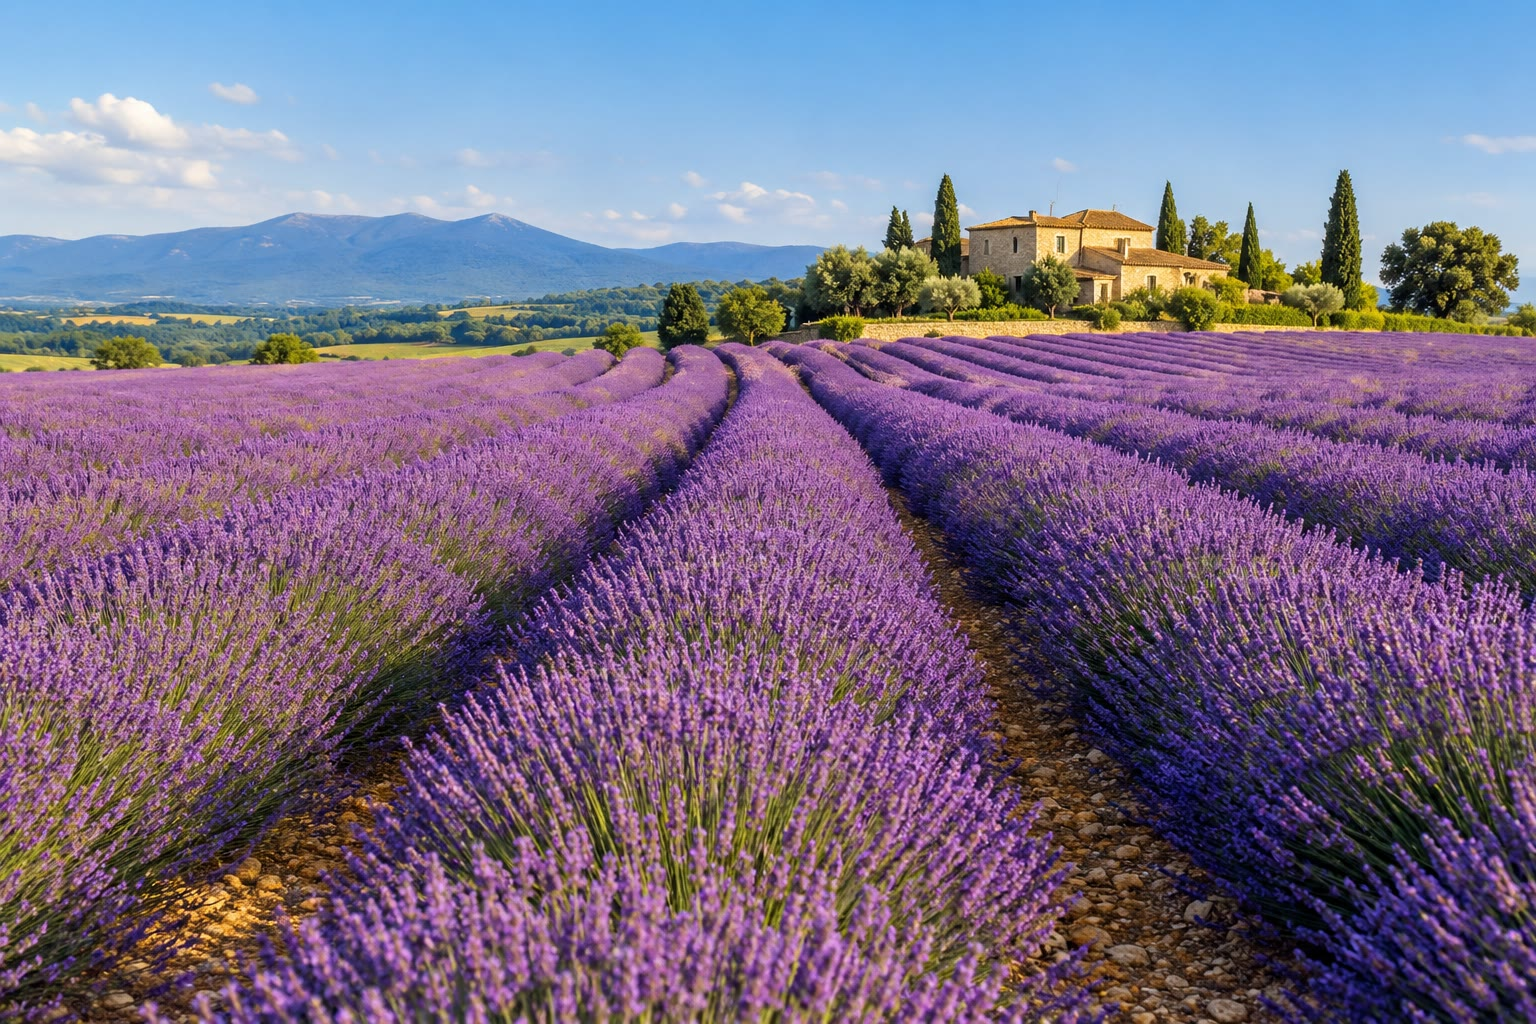
\includegraphics[width=0.55\linewidth]{images/book1/ai/g10-lavender-field.jpg}

{\small Un campo de lavanda en flor: la \omterm{def:g5:raw-materials-and-recycling:raw-material}{materia prima} del aceite esencial
de lavanda.}
\end{omfigure}

\section{Ejercicios}

\begin{exercise}[$\star$]\label{exo:g10:chemical-species:1}
¿\omterm{def:g10:chemical-species:natural}{Especie natural} o sintética? La vainillina de una vaina de vainilla; la
aspirina; la cafeína de los granos de café; la vainillina fabricada en
una fábrica.
\end{exercise}

\begin{exercise}[$\star$]\label{exo:g10:chemical-species:2}
¿Por qué la vainillina sintética y la vainillina natural tienen el mismo
punto de fusión?
\end{exercise}

\begin{exercise}[$\star$]\label{exo:g10:chemical-species:3}
En una placa de CCF, el frente del \omterm{def:g10:chemical-species:tlc}{eluyente} está a \qty{6.0}{cm} por
encima de la línea de partida y una mancha está a \qty{2.4}{cm} por
encima de ella. Calcula su $R_f$.
\end{exercise}

\begin{exercise}[$\star$]\label{exo:g10:chemical-species:4}
Da el papel del refrigerante en una \omterm{def:g10:chemical-species:distillation}{destilación}, y di por qué el agua
fría entra por su extremo inferior.
\end{exercise}

\begin{exercise}[$\star$]\label{exo:g10:chemical-species:5}
Nombra las tres condiciones que debe cumplir un \omterm{def:g6:solutions-and-solubility:solute}{disolvente} de
\omterm{def:g10:chemical-species:extraction}{extracción}.
\end{exercise}

\begin{exercise}[$\star\star$]\label{exo:g10:chemical-species:6}
Con la tabla de \omterm{def:g6:solutions-and-solubility:solute}{disolventes}, explica por qué no se puede usar el etanol
para extraer el linalol del destilado, y en cambio sí el ciclohexano.
\end{exercise}

\begin{exercise}[$\star\star$]\label{exo:g10:chemical-species:7}
En un embudo de \omterm{def:g3:separating-mixtures:decant}{decantación} se agita diclorometano con agua. ¿Qué capa
queda arriba? Justifícalo con la tabla.
\end{exercise}

\begin{exercise}[$\star\star$]\label{exo:g10:chemical-species:8}
Un polvo blanco vendido como aspirina empieza a fundir a
\qty{126}{\celsius} y está totalmente fundido a \qty{132}{\celsius}.
¿Qué puedes concluir?
\end{exercise}

\begin{exercise}[$\star\star$]\label{exo:g10:chemical-species:9}
Mira la figura de la CCF de este capítulo. ¿Qué contiene el aceite de
lavanda? ¿Qué especie subió más alto?
\end{exercise}

\begin{exercise}[$\star\star$]\label{exo:g10:chemical-species:10}
Ordena los pasos para obtener aceite de lavanda en el laboratorio:
separar las capas; \omterm{def:g10:chemical-species:distillation}{hidrodestilación}; añadir ciclohexano al destilado y
agitar; \omterm{def:g3:separating-mixtures:evaporate}{evaporar} el ciclohexano.
\end{exercise}

\begin{exercise}[$\star\star$]\label{exo:g10:chemical-species:11}
¿Por qué la línea de partida de una placa de CCF se traza con lápiz y se
sitúa por encima del \omterm{def:g10:chemical-species:tlc}{eluyente}?
\end{exercise}

\begin{exercise}[$\star\star\star$]\label{exo:g10:chemical-species:12}
Después de la \omterm{def:g10:chemical-species:extraction}{extracción}, el ciclohexano se elimina calentando
suavemente, y queda el aceite. Con los puntos de ebullición del
ciclohexano y del linalol (\qty{198}{\celsius}), explica por qué esto funciona.
\end{exercise}

\begin{exercise}[$\star\star\star$]\label{exo:g10:chemical-species:13}
Una muestra sintética de un aroma da una sola mancha en una placa de
CCF, a la altura de la \omterm{def:g10:chemical-species:natural}{especie natural}, y funde de forma neta a la
temperatura correcta. ¿Qué dos conclusiones puedes sacar?
\end{exercise}

\begin{exercise}[$\star\star\star$]\label{exo:g10:chemical-species:14}
En la misma CCF, la mancha A tiene $R_f = 0.40$ y el frente está a
\qty{5.5}{cm} por encima de la línea. ¿A qué altura está la mancha A?
Otra especie tiene $R_f = 0.75$: ¿a qué distancia por encima de la
mancha A está?
\end{exercise}

\begin{exercise}[$\star\star\star$]\label{exo:g10:chemical-species:15}
En \qty{1}{L} de agua se pueden \omterm{def:g2:mixing-and-dissolving:dissolve}{disolver} \qty{1.6}{g} de linalol. Un
destilado de \qty{200}{mL} de agua contiene \qty{0.20}{g} de linalol
disuelto. ¿Está saturado? ¿Cuánto más podría \omterm{def:g2:mixing-and-dissolving:dissolve}{disolver}? ¿Por qué merece la
pena extraer esta agua con ciclohexano en lugar de tirarla?
\end{exercise}

\clearpage % mantiene el título junto al recuadro del problema (quedaba aislado al pie de una página)
\section{Problema: El aroma de la lavanda}

\begin{problem}[{Problema de fin de semana --- de una cesta de flores de
lavanda a unas gotas de aceite esencial, comprobadas por cromatografía}]
\label{pb:g10:chemical-species:1}
% ledger: rho:cyclohexane, bp:cyclohexane, rho:CH2Cl2, bp:linalool, ghs:cyclohexane
En el laboratorio de un instituto se hidrodestilan con agua \qty{100}{g}
de flores de lavanda frescas. El destilado, turbio, se agita con
\qty{20}{mL} de ciclohexano en un embudo de \omterm{def:g3:separating-mixtures:decant}{decantación}; se conserva la
capa de ciclohexano, se seca, y el ciclohexano se \omterm{def:g3:separating-mixtures:evaporate}{evapora} calentando
suavemente. Lo que queda es aceite esencial de lavanda. Usa la tabla de
\omterm{def:g6:solutions-and-solubility:solute}{disolventes} de este capítulo.

\medskip
\noindent\textbf{Parte I --- La \omterm{def:g10:chemical-species:distillation}{hidrodestilación}.}
\begin{enumerate}
  \item ¿Cuál es el papel del agua hirviendo en una \omterm{def:g10:chemical-species:distillation}{hidrodestilación}?
  \item ¿Cuál es el papel del refrigerante? ¿Por dónde entra en él el
        agua fría?
  \item El destilado presenta una fina capa aceitosa que flota sobre el
        agua. ¿Es el aceite \omterm{def:g6:solutions-and-solubility:miscible}{miscible} con el agua? ¿Es más o menos denso
        que el agua?
  \item ¿Por qué no se vierte simplemente el destilado para recuperar el
        aceite?
\end{enumerate}

\medskip
\noindent\textbf{Parte II --- La \omterm{def:g10:chemical-species:extraction}{extracción}.}
\begin{enumerate}[resume]
  \item ¿Por qué el ciclohexano es un \omterm{def:g6:solutions-and-solubility:solute}{disolvente} adecuado para esta
        \omterm{def:g10:chemical-species:extraction}{extracción}?
  \item ¿Se podría usar etanol en su lugar? Explícalo.
  \item Después de agitar y dejar reposar, ¿la capa de ciclohexano queda
        arriba o abajo? ¿Y si fuera diclorometano?
  \item Da dos precauciones que exigen los pictogramas del ciclohexano.
  \item ¿Por qué se puede \omterm{def:g3:separating-mixtures:evaporate}{evaporar} el ciclohexano sin perder el linalol, que hierve a \qty{198}{\celsius}?
\end{enumerate}

\medskip
\noindent\textbf{Parte III --- La cromatografía.}
Se ponen en una placa de CCF manchas del aceite, de linalol puro (L) y
de etanoato de linalilo puro (A). Después del desarrollo, el frente está
a \qty{6.0}{cm} por encima de la línea de partida. El aceite da dos
manchas, a \qty{2.4}{cm} y a \qty{4.5}{cm}; la mancha L está a
\qty{2.4}{cm}, y la mancha A, a \qty{4.5}{cm}.
\begin{enumerate}[resume]
  \item Calcula el $R_f$ del linalol y el del etanoato de linalilo.
  \item ¿Qué contiene el aceite, según lo que muestra esta placa?
  \item ¿Es el aceite de lavanda una \omterm{def:g6:pure-substances-and-mixtures:pure-substance}{sustancia pura}?
  \item ¿Por qué se pusieron las referencias en la misma placa que el
        aceite?
  \item Se pone una mancha de un linalol sintético en otra placa
        desarrollada en las mismas condiciones: su mancha tiene
        $R_f = 0.40$. ¿Qué se puede concluir?
\end{enumerate}

\medskip
\noindent\textbf{Parte IV --- ¿Cuánto aceite?}
El aceite obtenido ocupa \qty{1.0}{mL}; \qty{1}{mL} de este aceite pesa
\qty{0.90}{g}.
\begin{enumerate}[resume]
  \item ¿Qué masa de aceite se ha obtenido?
  \item ¿Qué porcentaje de la masa de las flores es eso?
  \item ¿Qué masa de flores haría falta para obtener \qty{100}{g} de
        aceite?
  \item Se dice que el aceite es ``natural''. ¿En qué sentido es cierto?
        ¿Es su linalol distinto del linalol sintético?
  \item Indica la masa de aceite esencial que se obtiene a partir de
        \qty{100}{g} de flores.
\end{enumerate}
\end{problem}
